\documentclass[english,,man]{apa6}
\usepackage{lmodern}
\usepackage{amssymb,amsmath}
\usepackage{ifxetex,ifluatex}
\usepackage{fixltx2e} % provides \textsubscript
\ifnum 0\ifxetex 1\fi\ifluatex 1\fi=0 % if pdftex
  \usepackage[T1]{fontenc}
  \usepackage[utf8]{inputenc}
\else % if luatex or xelatex
  \ifxetex
    \usepackage{mathspec}
  \else
    \usepackage{fontspec}
  \fi
  \defaultfontfeatures{Ligatures=TeX,Scale=MatchLowercase}
\fi
% use upquote if available, for straight quotes in verbatim environments
\IfFileExists{upquote.sty}{\usepackage{upquote}}{}
% use microtype if available
\IfFileExists{microtype.sty}{%
\usepackage{microtype}
\UseMicrotypeSet[protrusion]{basicmath} % disable protrusion for tt fonts
}{}
\usepackage{hyperref}
\hypersetup{unicode=true,
            pdftitle={The Language of War: A Replication and Extension of Abe (2012) and Matsumoto et al. (2015)},
            pdfauthor={Kayla N. Jordan, Erin M. Buchanan, \& William E. Padfield},
            pdfkeywords={language, war, congress, pronouns, verbs},
            pdfborder={0 0 0},
            breaklinks=true}
\urlstyle{same}  % don't use monospace font for urls
\ifnum 0\ifxetex 1\fi\ifluatex 1\fi=0 % if pdftex
  \usepackage[shorthands=off,main=english]{babel}
\else
  \usepackage{polyglossia}
  \setmainlanguage[]{english}
\fi
\usepackage{graphicx,grffile}
\makeatletter
\def\maxwidth{\ifdim\Gin@nat@width>\linewidth\linewidth\else\Gin@nat@width\fi}
\def\maxheight{\ifdim\Gin@nat@height>\textheight\textheight\else\Gin@nat@height\fi}
\makeatother
% Scale images if necessary, so that they will not overflow the page
% margins by default, and it is still possible to overwrite the defaults
% using explicit options in \includegraphics[width, height, ...]{}
\setkeys{Gin}{width=\maxwidth,height=\maxheight,keepaspectratio}
\IfFileExists{parskip.sty}{%
\usepackage{parskip}
}{% else
\setlength{\parindent}{0pt}
\setlength{\parskip}{6pt plus 2pt minus 1pt}
}
\setlength{\emergencystretch}{3em}  % prevent overfull lines
\providecommand{\tightlist}{%
  \setlength{\itemsep}{0pt}\setlength{\parskip}{0pt}}
\setcounter{secnumdepth}{0}
% Redefines (sub)paragraphs to behave more like sections
\ifx\paragraph\undefined\else
\let\oldparagraph\paragraph
\renewcommand{\paragraph}[1]{\oldparagraph{#1}\mbox{}}
\fi
\ifx\subparagraph\undefined\else
\let\oldsubparagraph\subparagraph
\renewcommand{\subparagraph}[1]{\oldsubparagraph{#1}\mbox{}}
\fi

%%% Use protect on footnotes to avoid problems with footnotes in titles
\let\rmarkdownfootnote\footnote%
\def\footnote{\protect\rmarkdownfootnote}


  \title{The Language of War: A Replication and Extension of Abe (2012) and Matsumoto et al. (2015)}
    \author{Kayla N. Jordan\textsuperscript{1}, Erin M. Buchanan\textsuperscript{2}, \& William E. Padfield\textsuperscript{2}}
    \date{}
  
\shorttitle{LANGUAGE OF WAR}
\affiliation{
\vspace{0.5cm}
\textsuperscript{1} University of Texas - Austin\\\textsuperscript{2} Missouri State University}
\keywords{language, war, congress, pronouns, verbs}
\usepackage{csquotes}
\usepackage{upgreek}
\captionsetup{font=singlespacing,justification=justified}

\usepackage{longtable}
\usepackage{lscape}
\usepackage{multirow}
\usepackage{tabularx}
\usepackage[flushleft]{threeparttable}
\usepackage{threeparttablex}

\newenvironment{lltable}{\begin{landscape}\begin{center}\begin{ThreePartTable}}{\end{ThreePartTable}\end{center}\end{landscape}}

\makeatletter
\newcommand\LastLTentrywidth{1em}
\newlength\longtablewidth
\setlength{\longtablewidth}{1in}
\newcommand{\getlongtablewidth}{\begingroup \ifcsname LT@\roman{LT@tables}\endcsname \global\longtablewidth=0pt \renewcommand{\LT@entry}[2]{\global\advance\longtablewidth by ##2\relax\gdef\LastLTentrywidth{##2}}\@nameuse{LT@\roman{LT@tables}} \fi \endgroup}


\DeclareDelayedFloatFlavor{ThreePartTable}{table}
\DeclareDelayedFloatFlavor{lltable}{table}
\DeclareDelayedFloatFlavor*{longtable}{table}
\makeatletter
\renewcommand{\efloat@iwrite}[1]{\immediate\expandafter\protected@write\csname efloat@post#1\endcsname{}}
\makeatother
\usepackage{lineno}

\linenumbers

\authornote{Kayla N. Jordan is a Ph.D.~candidate at the University of Texas at Austin. Erin M. Buchanan is an Associate Professor of Quantitative Psychology at Missouri State University. William E. Padfield is a Masters degree candidate at Missouri State University.

Correspondence concerning this article should be addressed to Kayla N. Jordan, 108 E Dean Keeton St, Austin, TX 78712. E-mail: \href{mailto:kaylajordan@utexas.edu}{\nolinkurl{kaylajordan@utexas.edu}}}

\abstract{
Legislative bodies have very important roles and understanding the psychology of their decision-making processes is a useful area of study. We add to this area by replicating two previous studies Abe (2012) and Matsumoto, Frank, and Hwang (2015) in the context of a legislative body. The present study hypothesized that legislators who support war measures be externally focused and less cognitively complex in their speeches while opponents of war measures would be internally focused. Speeches were obtained pertaining to the decisions for the U.S. to take military action in Kosovo, Iraq, and Libya. While we found mixed results depending on the circumstances of a specific conflict, we demonstrate how automated language analysis can be combined with voting records to better understand behavioral action, such as legislative decision.


}

\begin{document}
\maketitle

In the last few years, numerous civil disputes worldwide, which might threaten American interests and human rights, have spurred considerable debate over American military intervention. Despite declines in legislative control of foreign policy, the U.S. Congress still plays an important role in deciding how the military is used by retaining the rights to formally declare war, limit the use of military force, and control military appropriations (Phelps \& Boylan, 2002). Previous research examined the predictors of presidential use of military force (Clark \& Nordstrom, 2005; Keller \& Foster, 2012) and predictors of public support for war (Cohrs \& Moschner, 2002; Friese, Fishman, Beatson, Sauerwein, \& Rip, 2009; McCleary, Nalls, \& Williams, 2009). However, the predictors of legislative support of military action have been understudied, thus presenting an interesting opportunity for exploration as well as replication of past studies in new contexts (Kriner \& Shen, 2014).

In this study, we sought to replicate two studies of the role of linguistic style in predicting war attitudes and behaviors, Abe (2012) and Matsumoto et al. (2015). Rather than use what people were thinking about, these studies focused on how people were thinking about the issues surrounding war freeing the investigation from issues of context as well as allowing a more psychological understanding of the process of conflict decisions and rationalizations. Abe (2012) analyzed the cognitive styles and attentional focus of online discussions of the Iraq War finding supporters of the war tended to have an external focus while opponents tended to have an internal focus. Those without a strong stance on the war exhibited greater cognitive complexity. Matsumoto et al. (2015) analyzed the same linguistic constructs for texts of world leaders preceding acts of aggression, such as wars or bombings, finding similar results with higher external focus and lower cognitive complexity preceding aggressive acts. In our replication of these studies, we analyze the same linguistic constructs in the context of a legislative body (i.e.~U.S. Congress) voting on war measures.

\hypertarget{psychological-language-analysis}{%
\subsection{Psychological Language Analysis}\label{psychological-language-analysis}}

Language, including political rhetoric, is the fusion of content and style words. Within any given sample of language, content words answer the question of what is being said, while style words answer the question of how it is being said. Content words include nouns, verbs, and adjectives, and style words include pronouns, prepositions, articles, conjunctions, negations, and quantifiers (Pennebaker, 2011). The Linguistic Inquiry and Word Count program (LIWC2007; Pennebaker, Booth, \& Frances, 2007) is text analysis software developed to summarize these types of words by breaking them down into 82 language categories. Besides style words, the LIWC measures constructs including: a) cognitive processes, such as \emph{know}, \emph{because}, and \emph{none} reflecting causation, exclusivity, and certainty, b) emotionality, which include words such as \emph{happy}, \emph{sad}, and \emph{angry}, c) relativity, such as \emph{go}, \emph{down}, and \emph{until} reflecting motion, space, and time, and d) personal concerns like money, death, and religion among others.

In many fields including social psychology, the LIWC analysis has become a common way to better understand psychological processes through the words people use. Tausczik and Pennebaker (2010) reviewed over 100 articles that used language as a basis for studying other constructs; specifically, these studies investigated how categories in the LIWC are related to psychological phenomena, such as attention, dominance, and deception. In the current investigation, we focus on attention as a potential mechanism for understanding how legislator's might work through decisions about war.

Just as a person's gaze can illuminate where their attention is so can the words they use. Specifically, pronouns and verb tense can demonstrate attentional focus by indicating who or what someone is attending to in a situation and how they are processing the situation. Therefore, greater use of first person pronouns indicated a self-focus, third person pronouns indicated a focus on others, and verb tense indicated whether the focus was on past, present, or future events (Tausczik \& Pennebaker, 2010). Attentional focus in the form of pronouns has been linked to depression (Rude, Gortner, \& Pennebaker, 2004), bullying (Kowalski, 2000), and marital satisfaction (Simmons, Gordon, \& Chambless, 2005). In the studies we seek to replicate, Abe (2012) found supporters of the war tended to have an external focus, using more third person pronouns, while opponents of the war tended to have an internal focus, using more first person pronouns. Matsumoto et al. (2015) also found greater use of plural third person pronouns (i.e., \emph{we}, \emph{us}) predicted aggressive acts by groups by examining historical texts.

Another construct which can be automatically measured from language is cognitive complexity. Originally developed by ({\textbf{???}}), cognitive complexity measures the extent to which people are drawing distinctions between concepts and integrating ideas. In past studies, cognitive complexity has been found to be related to individual differences measures such as extraversion and conscientiousness ({\textbf{???}}), aggressive behaviors (Pennebaker, 2011), and reactions to negative events (Abe, 2011). Most relevant to the current study, Matsumoto et al. (2015) found cognitive complexity to decrease immediately before acts of aggression which is the effect we wish to replicate.

The purpose of the current studies is to determine if past studies on war decisions and aggression replicate in the context of the U.S. Congress when voting on war measures.

\hypertarget{hypotheses}{%
\subsection{Hypotheses}\label{hypotheses}}

H1: Legislators supporting war measure will have an external focus and use more 3rd person pronouns (particularly 3rd person plural pronouns) (Abe, 2012; Matsumoto et al., 2015).

H2: Legislators opposing war measure will have an internal focus and use more 1st person pronouns (Abe, 2012).

H3: Legislators supporting wars measure will exhibit lower cognitive complexity than those opposing the measure (Matsumoto et al., 2015).

\hypertarget{method}{%
\section{Method}\label{method}}

\hypertarget{language-samples}{%
\subsection{Language Samples}\label{language-samples}}

Linguistic frequency analysis was conducted on political speeches gleaned from Congress. The source of language samples was the Congressional Record, a searchable database containing a record of each session of Congress since 1995 available at \url{https://www.congress.gov/congressional-record}, which is maintained by the U.S. Government Publishing Office. For this study, we searched for pertinent speeches from January 27, 1998 to September 19, 2013. Records were included if they pertained to U.S. relations with the following countries: Iraq, Libya, and Kosovo (see below for explanation of country selection). Samples were split by session date and person speaking, and therefore, each person could be represented multiple times in the dataset. Each file in the Congressional Record includes all speeches from the day selected, therefore, we separated each person's speeches by day into different files for processing. For example, a Senator may respond back and forth with an invited guest speaker, and all the Senators spoken words would be combined into one file for that day. Only Senators and Representatives were included in this analysis. These speeches were then coded for party affiliation of the Congressperson. All processed data, as well as an \emph{R} markdown document with data analysis scripts inline with this manuscript (Aust \& Barth, 2017) can be found at \url{https://osf.io/r8qp2/}.

\hypertarget{variables}{%
\subsection{Variables}\label{variables}}

\hypertarget{language}{%
\subsubsection{Language}\label{language}}

Each language sample was analyzed using the Language Inquiry and Word Count (Pennebaker et al., 2007). The LIWC provides percentages of each individual text that fall into each category of words. We examined pronouns for Hypotheses 1 and 2. The pronouns category included first person singular and plural pronouns (\emph{I, me, we}), second person pronouns (\emph{you, your}), and third person singular and plural pronouns (\emph{he, she, they}). To measure external focus, third person singular and third person plural pronouns were added together. To measure internal focus, first person pronouns both singular and plural were added together. For Hypothesis 3, cognitive complexity was calculated using the same formula as Abe (2012). The LIWC categories of exclusives, negations, tentative words, and conjunctions were z-scored and summed together.

\hypertarget{military-action}{%
\subsubsection{Military Action}\label{military-action}}

For the purpose of this study, military action was defined as military personnel being sent into another nation to coerce the actions of that nation. In the past 15 years, the U.S. has taken military action against Iraq, Afghanistan, Kosovo, and Libya, although Congress did not explicitly approve action in Afghanistan or Libya. Operational definitions for support for war were voting records (yay, nay) on bills authorizing military action for Iraq, Kosovo, and Libya (only voted on in the House). These bills were House Joint Resolution 114, 107th Congress (2002); Senate Concurrent Resolution 21, 106th Congress (1999); and House Joint Resolution 68, 112th Congress (2011). Oppose or support information was combined with the LIWC percentages described above.

\hypertarget{data-analytic-technique}{%
\subsection{Data Analytic Technique}\label{data-analytic-technique}}

The data collected include multiple language samples by the same senator and are structured by both party affiliation and region of interest. This structure was best analyzed with multilevel modeling, which allowed us to control for the correlated error terms of senator and party. We used the \emph{nlme} package to calculate the means and standard deviation for each variable by voting recording (Pinheiro, Bates, Debroy, Sarkar, \& Team, 2017). The intercept was used to predict the dependent variable (LIWC category percent), which creates a mean score for the dependent variable. Party affiliation and Congressperson name were controlled as random intercept factors (Gelman, 2006). The standard error of the estimate was translated into standard deviation by multiplying by the square root of n for the sample. This analysis was bootstrapped using the \emph{boot} library 1000 times, and the normal confidence interval for the mean was calculated using this function (Canty \& Ripley, 2017). These values were separated by voting record, Senate/House, and country of interest. The means and confidence intervals are presented in forest plots to show the relative percentages for each combination. The bootstrapped standard deviation values were used to calculate \(d_s\) values using the MOTE library with the pooled standard deviation as the denominator (Buchanan, Valentine, \& Scofield, 2017; Lakens, 2013).

\begin{table}[tbp]
\begin{center}
\begin{threeparttable}
\caption{\label{tab:Ktable}Descriptive statistics for each dependent variable by chamber, 
          region, and military support for Kosovo}
\small{
\begin{tabular}{lccccccccc}
\toprule
Chamber & Region & DV & $M_O$ & $SD_O$ & $M_S$ & $SD_S$ & $d_s$ & $d_s$ LL & $d_s$ UL\\
\midrule
House & Kosovo & i & 1.84 & 1.16 & 2.34 & 1.61 & -0.36 & -0.63 & -0.08\\
House & Kosovo & we & 3.12 & 1.56 & 2.91 & 2.06 & 0.11 & -0.16 & 0.39\\
House & Kosovo & shehe & 0.51 & 0.54 & 0.56 & 0.71 & -0.08 & -0.35 & 0.20\\
House & Kosovo & they & 0.66 & 0.56 & 0.80 & 0.98 & -0.18 & -0.45 & 0.09\\
House & Kosovo & complex & 0.62 & 2.50 & -0.55 & 3.05 & 0.62 & 0.34 & 0.90\\
House & Kosovo & internal & 4.95 & 2.01 & 5.27 & 2.74 & -0.13 & -0.40 & 0.14\\
House & Kosovo & external & 1.15 & 0.88 & 1.34 & 1.14 & -0.19 & -0.47 & 0.08\\
Senate & Kosovo & i & 2.19 & 1.16 & 1.96 & 1.78 & 0.15 & -0.41 & 0.71\\
Senate & Kosovo & we & 3.13 & 1.89 & 1.54 & 0.57 & 1.18 & 0.56 & 1.78\\
Senate & Kosovo & shehe & 0.44 & 0.82 & 0.47 & 0.40 & -0.05 & -0.61 & 0.51\\
Senate & Kosovo & they & 0.79 & 0.62 & 0.53 & 0.36 & 0.51 & -0.06 & 1.08\\
Senate & Kosovo & complex & 0.14 & 9.11 & -1.47 & 2.41 & 0.25 & -0.31 & 0.81\\
Senate & Kosovo & internal & 5.31 & 2.24 & 3.54 & 1.93 & 0.85 & 0.26 & 1.43\\
Senate & Kosovo & external & 1.22 & 1.14 & 1.04 & 0.60 & 0.21 & -0.35 & 0.77\\
\bottomrule
\addlinespace
\end{tabular}
}
\begin{tablenotes}[para]
\normalsize{\textit{Note.} Confidence intervals for $d_s$ were calculated using 
          non-central $t$ distribution. O = Oppose, S = Support, LL = Lower Limit, UL = Upper Limit.}
\end{tablenotes}
\end{threeparttable}
\end{center}
\end{table}

\begin{verbatim}
## Warning: Removed 9 rows containing missing values (geom_pointrange).

## Warning: Removed 9 rows containing missing values (geom_pointrange).
\end{verbatim}

\begin{verbatim}
## Warning: Removed 10 rows containing missing values (geom_pointrange).
\end{verbatim}

\begin{figure}
\centering
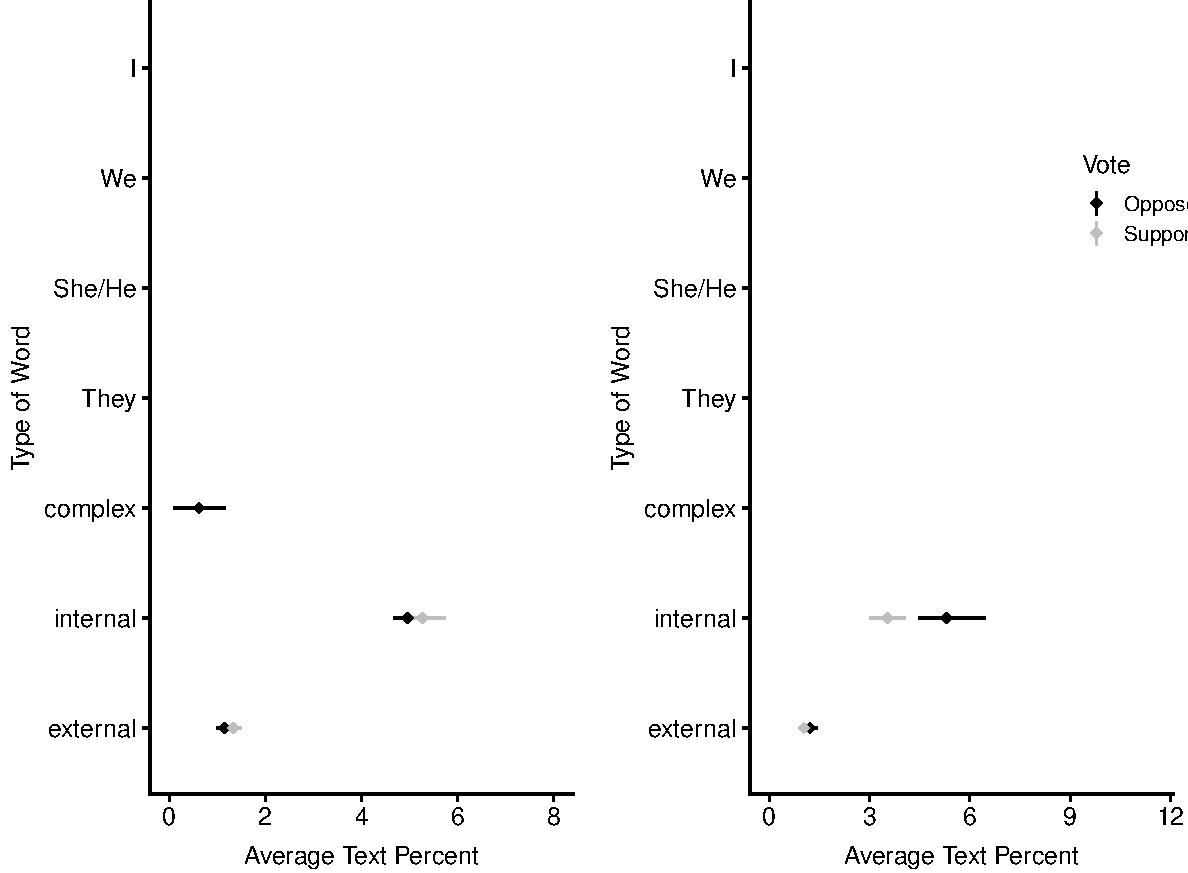
\includegraphics{Language_of_War_Markdown_KJ2_files/figure-latex/Kpic-1.pdf}
\caption{\label{fig:Kpic}House (left) and Senate (right) bootstrapped means and 95\% confidence interval for pronouns and verb tenses for Kosovo.}
\end{figure}

\hypertarget{study-1a---kosovo-in-the-house}{%
\section{Study 1A - Kosovo in the House}\label{study-1a---kosovo-in-the-house}}

In early 1998, violence erupted in the Serbian region of Kosovo between ethnic Albanians and the Serbian government. A peace agreement later in the year lasted until the beginning of 1999 when several Albanian civilians were killed, prompting a resurrection of hostilities. When the Serbian government, namely President Slobodan Milosevic, failed to concede to allowing a NATO peacekeeping force in Kosovo during February 1999 negotiations, NATO authorized air strikes against Serbian targets. This decision subsequently prompted debate within the U.S. Congress as to the involvement of the U.S. military in NATO's operations in Serbia and Kosovo (Woehrel \& Kim, 2006).

In this study, we examine this debate in the U.S. House of Representatives to determine if members of Congress who supported U.S. military involvement focused on people or events differently than those who opposed it.

\hypertarget{method-1}{%
\section{Method}\label{method-1}}

Speeches made in the House of Representatives pertaining to the use of military force in Kosovo/Serbia were gathered from the Congressional Record available from the U.S. Government Publishing Office. In total, 210 speeches were collected. Speeches were limited to those made in the year preceding the vote on Senate Concurrent Resolution 21 made on April 28, 1999 to allow the President to conduct air and missile strikes against Yugoslavia (Serbia and Montenegro). This resolution failed in the House with 213-213 with 86\% of Democrats supporting the resolution and 84\% of Republicans opposing. These speeches were made by 156 unique speakers where where Republicans gave 108 speeches, Democrats gave 98 speeches, one Independent, one Non-Partisan, and two non-Representatives. Five speeches were excluded for no voting record. The average word count was 700.51 (\emph{SD} = 814.04).

\hypertarget{results}{%
\section{Results}\label{results}}

A forest plot of the results can be found in Figure \ref{fig:Kpic}, and all descriptive statistics can be found in Table \ref{tab:Ktable}. Results only weakly supported Hypothesis 1. The trend is in the hypothesized direction with supporters of military action displaying greater external focus, but the effect is non-significant. Hypothesis 2 was not supported; legislators opposing the war measure did not display a greater internal focus. In fact, supporters of the measure used more 1st person singular pronouns (e.g.~I-words) contrary to our hypothesis. Hypothesis 3 was supported with supporters of the war measure showing lower cognitive complexity than those who opposed it.

\hypertarget{study-1b---kosovo-in-the-senate}{%
\section{Study 1B - Kosovo in the Senate}\label{study-1b---kosovo-in-the-senate}}

In the second part of this study, we examined the Kosovo debate in the U.S. Senate to determine if the differences found in the first part of the study replicate in a slightly different context.

\hypertarget{method-2}{%
\section{Method}\label{method-2}}

Speeches were gathered in the same manner as in the first part of the study. All speeches made in the Senate in the year before the March 23, 1999 vote on Senate Concurrent Resolution 21. This resolution passed the Senate with 58 supporting and 41 opposing. All but 3 Democrats supported the resolution while 70\% of Republicans opposed it. A total of 49 speeches were collected. These speeches were made by 25 unique senators with 12 speeches by Democrats and 37 by Republicans. The average word count for these speeches was 1413.14 (\emph{SD} = 1076.37).

\hypertarget{results-1}{%
\section{Results}\label{results-1}}

Analyses were conducted in the same manner as the first part of the study with bootstrapped means and CIs calculated for the seven categories marking attention. Results can be seen as a forest plot in Figure \ref{fig:Kpic} and Table \ref{tab:Ktable}. For the Senate, Hypothesis 1 was not supported. No significant differences in external focus or 3rd person plural pronouns were found. Hypothesis 2 was supported with legislators opposing the war measure displaying a much higher internal focus than legislators supporting the war measure. Hypothesis 3 was partially supported. While not statistically significant, supporters of the war measure tended to show lower cognitive complexity than those who opposed it.

\hypertarget{discussion}{%
\section{Discussion}\label{discussion}}

The results of this first study only consistently support Hypothesis 3 (supporters of war measures would be less cognitively complex). The results were inconsistent for Hypothesis 1 and 2 (supporters of war measures would be more externally focus while those opposing would be internally focused) in that effects found for the House and Senate are non-overlapping. For Hypothesis 1, supporters of war in the House were marginally more externally focused but the effect was not replicated for the Senate. For Hypothesis 2, those opposing the measure in the Senate were more internally focused, but the same could not be said for those in the House.
It is difficult to know exactly why this is the case; however there are several possible explanations. First, voting in Congress is exceedingly complex and is influenced by much more than floor debates in a given chamber. In this case, the Senate vote on the resolution occurred before the main debate in the House, which may have influenced what the debate focused on. Second, the Senate and the House are composed differently. Members of the House serve two year terms while Senators serve six year terms. Furthermore, Senators typically have more political experience than members of the House. These, as well as other factors, may help explain the differential effects for the two chambers of Congress.

Based on the findings of Abe (2012) and Matsumoto et al. (2015), we expected more consistent support for our hypotheses. However, the results could also be explained by the situation posed by the particular resolution. In this conflict, rather than responding to an act of aggression or a perceived threat, the U.S. was deciding the extent to which the U.S. would be involved in ongoing NATO (a treaty organization of which the U.S. is a member) operations in Kosovo and Serbia. It is possible that some viewed the outgroup as NATO rather than Serbians. In this case, with no clear, immediate threat to the U.S., for those making ingroup-outgroup distinctions, protecting the ingroup may have meant opposing the war rather than supporting it. In order to determine if the situation surrounding the Kosovo conflict may have impacted the first study, we next turned to examine the Iraq War which was had more support and also represented a possible clear threat to the U.S.

\hypertarget{study-2a---iraq-in-the-house}{%
\section{Study 2A - Iraq in the House}\label{study-2a---iraq-in-the-house}}

In this next study, we examined the debate preceding the congressional approval of the use of military force against Iraq. Regime change had been a long-standing position of the U.S. toward Iraq following the Gulf War; however serious military action was not considered until after the World Trade Center attacks on September 11, 2001. In 2002, President Bush declared Iraq part of an \enquote{axis of evil} in his State of the Union address. Iraq's repeated violations of nuclear arms agreements, ties to terrorist organizations, and pursuit of weapons of mass destruction were argued by the Bush Administration to potentially pose a major threat to U.S. national security. This prompted the debate within Congress as to whether or not to approve President Bush's request for military action (Katzman, 2002). These studies were used to determine if the findings from the first study extend to a different conflict. Specifically, in the first part of this study, we examined the debate in the House of Representatives to determine if members of Congress who supported taking military action used more self and future references.

\hypertarget{method-3}{%
\section{Method}\label{method-3}}

Once again using the Government Publishing Office, we collected speeches given in the House of Representatives pertaining to the use of U.S. military force against Iraq in the three months before the vote on House Joint Resolution 114 on October 10, 2002. This bill passed the House with a 296-133 majority; with most Republicans supporting the measure and 60\% of Democrats opposing. A total of 274 speeches were collected representing 233 unique speakers. Of these speeches, 155 speeches were made by Democrats, 119 were made by Republicans. The average word count of the speeches was 742.34 (\emph{SD} = 1053.45). Four speeches were excluded for no voting record.

\hypertarget{results-2}{%
\section{Results}\label{results-2}}

\begin{table}[tbp]
\begin{center}
\begin{threeparttable}
\caption{\label{tab:Itable}Descriptive statistics for each dependent variable by chamber, 
          region, and military support for Iraq}
\small{
\begin{tabular}{lccccccccc}
\toprule
Chamber & Region & DV & $M_O$ & $SD_O$ & $M_S$ & $SD_S$ & $d_s$ & $d_s$ LL & $d_s$ UL\\
\midrule
House & Iraq & i & 1.66 & 1.33 & 1.90 & 2.15 & -0.13 & -0.37 & 0.11\\
House & Iraq & we & 3.01 & 1.61 & 2.76 & 1.37 & 0.17 & -0.07 & 0.41\\
House & Iraq & shehe & 0.56 & 0.56 & 1.16 & 0.92 & -0.77 & -1.02 & -0.52\\
House & Iraq & they & 0.46 & 0.51 & 0.49 & 1.36 & -0.03 & -0.27 & 0.21\\
House & Iraq & complex & 0.72 & 2.80 & -0.57 & 2.70 & 0.47 & 0.23 & 0.72\\
House & Iraq & internal & 4.66 & 1.98 & 4.59 & 1.82 & 0.03 & -0.21 & 0.28\\
House & Iraq & external & 1.03 & 0.82 & 1.71 & 1.08 & -0.70 & -0.95 & -0.45\\
Senate & Iraq & i & 1.99 & 1.25 & 1.98 & 1.60 & 0.01 & -0.36 & 0.37\\
Senate & Iraq & we & 2.47 & 0.97 & 2.61 & 1.15 & -0.13 & -0.50 & 0.23\\
Senate & Iraq & shehe & 0.60 & 0.47 & 1.20 & 0.62 & -1.03 & -1.42 & -0.65\\
Senate & Iraq & they & 0.49 & 0.32 & 0.56 & 0.40 & -0.19 & -0.55 & 0.18\\
Senate & Iraq & complex & 0.38 & 2.85 & -0.13 & 3.45 & 0.16 & -0.21 & 0.52\\
Senate & Iraq & internal & 4.47 & 1.47 & 4.60 & 1.82 & -0.08 & -0.44 & 0.29\\
Senate & Iraq & external & 1.08 & 0.62 & 1.76 & 0.81 & -0.89 & -1.26 & -0.50\\
\bottomrule
\addlinespace
\end{tabular}
}
\begin{tablenotes}[para]
\normalsize{\textit{Note.} Confidence intervals for $d_s$ were calculated using 
          non-central $t$ distribution. O = Oppose, S = Support, LL = Lower Limit, UL = Upper Limit.}
\end{tablenotes}
\end{threeparttable}
\end{center}
\end{table}

\begin{verbatim}
## Warning: Removed 9 rows containing missing values (geom_pointrange).

## Warning: Removed 9 rows containing missing values (geom_pointrange).
\end{verbatim}

\begin{verbatim}
## Warning: Removed 10 rows containing missing values (geom_pointrange).
\end{verbatim}

\begin{figure}
\centering
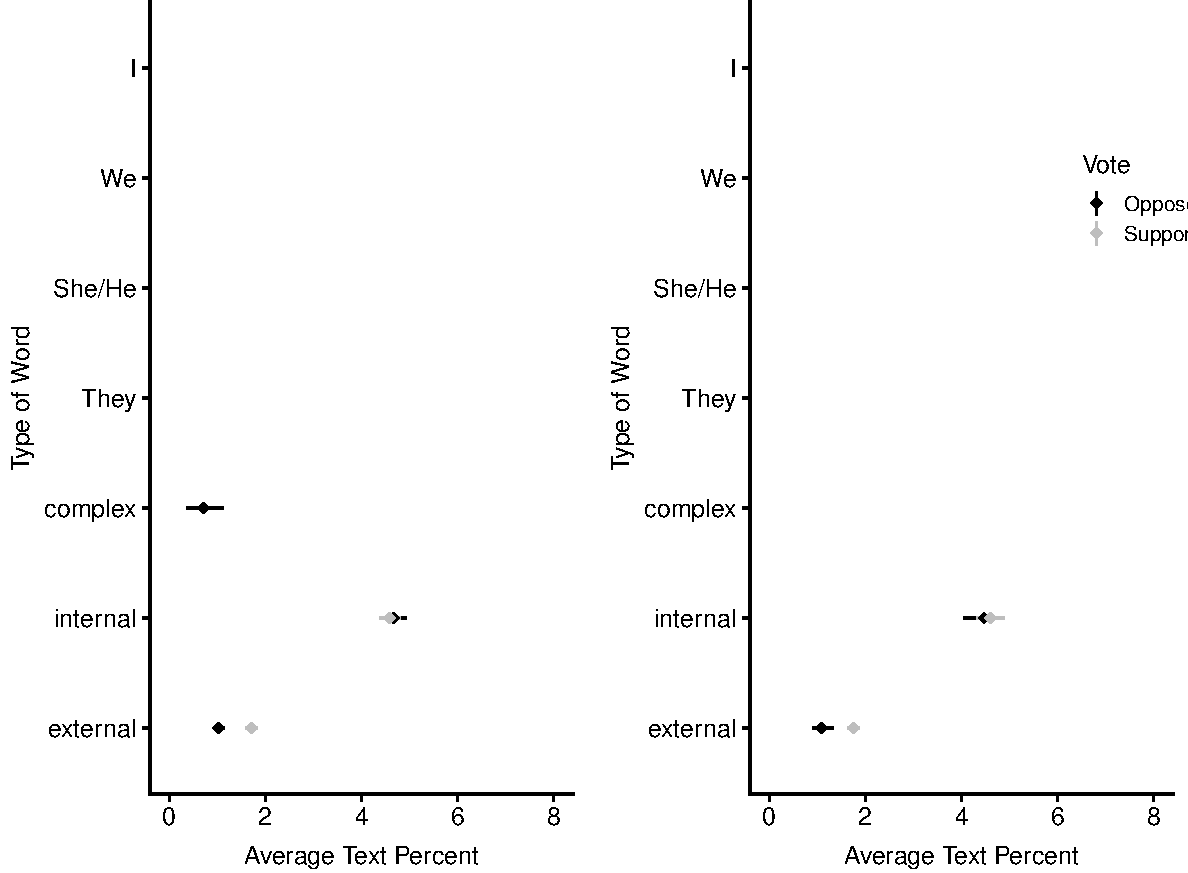
\includegraphics{Language_of_War_Markdown_KJ2_files/figure-latex/Ipic-1.pdf}
\caption{\label{fig:Ipic}House (left) and Senate (right) bootstrapped means and 95\% confidence interval for pronouns and verb tenses for Iraq.}
\end{figure}

As in the first study, bootstrapped means and confidence intervals as well as effect sizes (Cohen's \(d_s\)) were calculated for speeches of those supporting the measure versus those opposing the measure for the following LIWC categories: first-person singular (\emph{I}), first-person plural (\emph{we}), third-person singular (\emph{he}, \emph{she}), third-person plural (\emph{they}) as well as composite measure for external focus, internal focus, and cognitive complexity. Results can be seen as a forest plot in Figure \ref{fig:Ipic} and in Table \ref{tab:Itable}. Support was found for Hypothesis 1. Legislators supporting the war measure were more externally focused. However, rather than being primarily driven by third-person plural pronouns (\emph{they}), the largest differences was in third-person singular pronouns (\emph{he}). Hypothesis 2 was not supported; no significant difference was found in internal focus. Hypothesis 3 was supported; supporters of the war measure were significantly less cognitively complex than those who opposed it.

\hypertarget{study-2b---iraq-in-the-senate}{%
\section{Study 2B - Iraq in the Senate}\label{study-2b---iraq-in-the-senate}}

In the second part of this study, we examined the debate in the Senate. We wished to determine if, like senators who opposed military action in Kosovo, senators who opposed action against Iraq used more group references as well as more reference to current events or if senators were more like House members debating Iraq.

\hypertarget{method-4}{%
\section{Method}\label{method-4}}

In this part of the study, speeches from the Senate were gathered for the 6 months before the Senate vote on House Joint Resolution 114 conducted on October 11, 2002. The bill passed with a 77-23 majority. All but one Republican supported the measure as did 58\% of Democrats. In total, 138 speeches were collected representing 85 unique speakers. Of these speeches, 74 were given by Democrats and 64 by Republicans. The average word count for these speeches were 1991.23 (\emph{SD} = 1671.70).

\hypertarget{results-3}{%
\section{Results}\label{results-3}}

Analyses were conducted in the same manner as the first part of the study to determine differences between supporters and opponents of military action in Iraq in terms of the use of first-person singular (\emph{I}), first-person plural (\emph{we}), third-person singular (\emph{he}, \emph{she}), third-person plural (\emph{they}) as well as composite measure for external focus, internal focus, and cognitive complexity. Figure \ref{fig:Ipic} displays these results as a forest plot, and all values are in Table \ref{tab:Itable}. Hypothesis 1 was once again supported. Senators supporting the war legislations were more externally focus, and like in the House, tended to use third-person singular pronouns (\emph{he}) at higher rates. Once again, we failed to find support for Hypothesis 2 with no significant differences found in internal focus. Finally, while not statistically significant, cognitive complexity tended to be lower for Senators supporting the war measure providing at least partial support for Hypothesis 3.

\hypertarget{discussion-1}{%
\section{Discussion}\label{discussion-1}}

The results from this second study more closely matched our hypotheses. For both the House and Senate, members of Congress who supported taking military action were more externally focused than those who opposed taking military action. However contrary to our hypothesis, the difference in external focus was driven by third person singular pronouns (\emph{he}) rather than third person plural pronouns (\emph{they}). Although this finding was not quite the result we expected, these differences make sense in light of the situation. In the case of the Iraq War, the threat was seen not as a group of people but rather a single individual, Saddam Hussein. Hence, for supporters of military action, their focus was still external as was expected (Abe, 2012; Matsumoto et al., 2015); however, their focus was on an individual rather than a group.

The second hypothesis was not supported. In both the House and Senate, legislators who opposed the war measure were not more internally focused than those who supported it. As was stated previously, this difference in results could be due to voting procedures or compositional differences in the House and Senate. Finally, our third hypothesis was once again consistently supported. Those who supported the war measures showed less cognitive complexity than those who opposed them in both the House and Senate.

As a final test of our hypotheses, we examined the Congressional debate surrounding U.S. involvement in Libya during its 2011 civil war. We might expect to find similar results to Study 1 as, like the Kosovo war, there was less support for U.S. military involvement as well as a lack of a perceived clear, immediate threat to the U.S.

\hypertarget{study-3---libya-in-the-house}{%
\section{Study 3 - Libya in the House}\label{study-3---libya-in-the-house}}

In this final study, we examine the debate in the House of Representatives surrounding U.S. military involvement in Libya during its revolution. In February 2011, a revolt against Libyan dictator, Muammar Qaddafi, prompted the intervention of NATO when Qaddafi violently suppressed all opposition. The involvement of NATO lead to debate within Congress as to the exact role of the U.S. in military operations in Libya and the extent of U.S involvement (Blanchard, 2011). In examining this debate, we wished to determine if the language of those who supported or opposed military action was similar to those of either of the first two studies.

\hypertarget{method-5}{%
\section{Method}\label{method-5}}

In this final study, the Congressional Record was searched for speeches given in the House of Representatives pertaining to the debate of the authorization of military action against Libya in the three months before the vote on House Joint Resolution 68 on June 24, 2011. The bill failed in the House 123-295. All but 14 Republicans voted against the resolution while 60\% of Democrats supported the resolution. A total of 104 speeches were collected representing 76 unique speakers. Democrats made 53 of these speeches while 51 speeches were made by Republicans. The average word count for these speeches was 465.93 (\emph{SD} = 477.41). As the resolution failed in the House, it was not possible to examine this debate in the Senate. Five speeches were excluded for no voting record.

\hypertarget{results-4}{%
\section{Results}\label{results-4}}

\begin{table}[tbp]
\begin{center}
\begin{threeparttable}
\caption{\label{tab:Ltable}Descriptive statistics for each dependent variable by chamber, 
          region, and military support for Libya}
\small{
\begin{tabular}{lccccccccc}
\toprule
Chamber & Region & DV & $M_O$ & $SD_O$ & $M_S$ & $SD_S$ & $d_s$ & $d_s$ LL & $d_s$ UL\\
\midrule
House & Libya & i & 2.47 & 1.66 & 2.31 & 1.13 & 0.11 & -0.31 & 0.53\\
House & Libya & we & 3.08 & 2.22 & 2.89 & 1.87 & 0.09 & -0.33 & 0.51\\
House & Libya & shehe & 0.61 & 0.83 & 0.64 & 0.85 & -0.04 & -0.46 & 0.38\\
House & Libya & they & 0.60 & 0.91 & 0.64 & 0.72 & -0.04 & -0.46 & 0.37\\
House & Libya & complex & 0.34 & 3.25 & -0.75 & 3.09 & 0.34 & -0.08 & 0.76\\
House & Libya & internal & 5.34 & 1.75 & 5.17 & 2.00 & 0.09 & -0.32 & 0.51\\
House & Libya & external & 1.20 & 1.38 & 1.25 & 1.21 & -0.04 & -0.46 & 0.38\\
\bottomrule
\addlinespace
\end{tabular}
}
\begin{tablenotes}[para]
\normalsize{\textit{Note.} Confidence intervals for $d_s$ were calculated using 
          non-central $t$ distribution. O = Oppose, S = Support, LL = Lower Limit, UL = Upper Limit.}
\end{tablenotes}
\end{threeparttable}
\end{center}
\end{table}

\begin{figure}
\centering
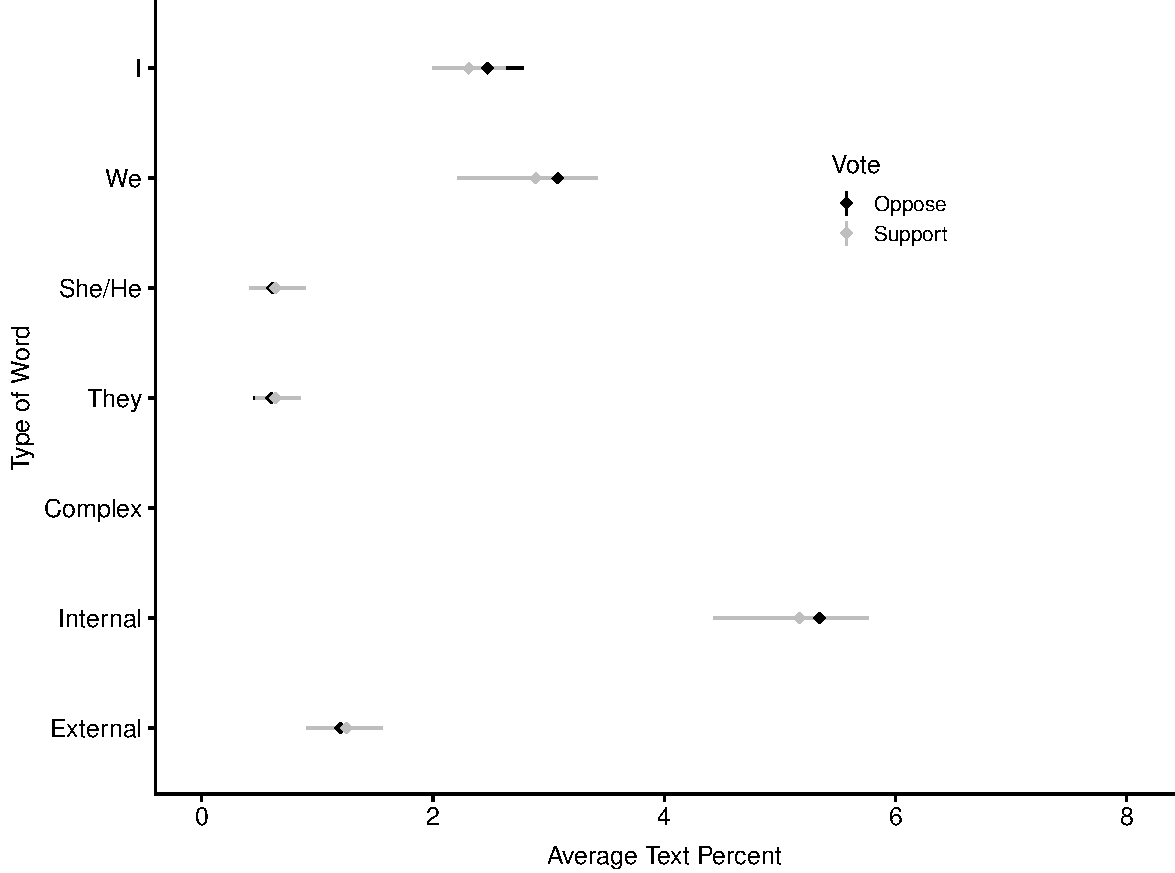
\includegraphics{Language_of_War_Markdown_KJ2_files/figure-latex/Lpic-1.pdf}
\caption{\label{fig:Lpic}House (left) and Senate (right) bootstrapped means and 95\% confidence interval for pronouns and verb tenses for Libya.}
\end{figure}

As in the first two studies, analyses consisted on comparing the bootstrapped means, CIs, and effects sizes for those who supported the military measure versus those who opposed it on the following linguistic measures: first-person singular (\emph{I}), first-person plural (\emph{we}), third-person singular (\emph{he}, \emph{she}), third-person plural (\emph{they}), past-tense, present-tense, and future tense. These results are displayed in Figure \ref{fig:Lpic} as a forest plot and in Table \ref{tab:Ltable}. No differences emerged on any measure.

\hypertarget{discussion-2}{%
\section{Discussion}\label{discussion-2}}

Though the evidence from this third study is somewhat weak, all three hypothesis were at least partially supported. The relatively small sample size limited the power of the study, but trends in each case were in the hypothesized direction. In addition to potentially limited power, our finding from Studies 1 and 3 could indicate that in situations where there is less Congressional support for military action and no clear, immediate threat to the U.S., the difference between support and opposition for military action is not a matter of attentional focus but rather other social and political forces.

\hypertarget{general-discussion}{%
\section{General Discussion}\label{general-discussion}}

Across all three studies, we found consistent, if somewhat weak evidence that supporters of war measures show less cognitive complexity in their speeches than those on the opposing side (Hypothesis 3) replicating part of the Matsumoto et al. (2015) study. When it comes to consideration of aggressive acts like war, our studies would suggest that legislators (at least in the U.S.) reason similarly to the executive leaders analyzed by Matsumoto et al. (2015). Political figures in favor of aggressive measures seek to simplify the debate whereas those against aggressive measure may seek to consider the issue more deeply. Whether the decreased cognitive complexity before aggression is a rhetorical strategy, ideological beliefs, cognitive style, or some other factor is worth further investigation.

Our hypotheses regarding internal and external focus were not consistently supported. Support for hypothesis 1 was found only in the case of the debate around the Iraq War. Interestingly, the Iraq War legislation was the only of our case in our three studies which received majority support in both the House and Senate. Differences in external focus may depend partially on the aggressive act having the support of the majority or having popular support or there being a potentially immediate, clear threat to the U.S. legislators could point to. In the cases of Kosovo and Libya, legislators may have supported the war measures for reasons other than aggression such as to support the president's agenda.

Hypothesis 2 received the least support of any of our hypothesis with significant differences found only in the Senate debate of the Kosovo resolution failing to replicate Abe (2012). Unlike Hypotheses 1 and 3 which are at least partially based in Matsumoto et al. (2015)\enquote{s study of executive, Hypothesis 2 is solely based in Abe (2012)'s study of the war attitudes of ordinary citizens. Our results suggest that findings of Abe (2012) may only generalize to laypeople and fail to capture the processes at work with the war decisions of political elites.
Additionally, we may have only partially replicated Matsumoto et al. (2015) is due to changes in the dynamics of war. While Matsumoto et al. (2015) examined events spanning 1830 to 2010, our study focused on three recent conflicts within the context of U.S. legislator bodies. Historically, the U.S. would declare war on another nation (i.e., fighting the Germans in WWI). In WWII, a slight shift occurred where the U.S. was fighting not only another nation but also an ideology (Nazi Germany, Fascist Italy). With the beginning of the Cold War, another movement happened where the U.S. did not directly fight another nation (USSR) but instead fought indirectly with proxy wars (Korean War, Vietnam War) while battling against enemy ideology (Communism). After the Cold War and the fall of the Soviet Union, the focus shifted to the United States} main conflict being the war on terror in which there is no nation to battle against just an idea (Matthews, 2014). Furthermore, Balas, Owsiak, and Diehl (2012) argued that one possible motivation for war, since the end of the Cold War, was the increased emphasis on the international norms of democratization and humanitarianism. Hence, rather than capturing solely support for aggressive actions, our study of congressional debates in this context may have also captured legislators' attitudes toward humanitarianism, globalization, and terrorism. Further work would be necessary to the different reasons why political figures might support or oppose a war measure.

\hypertarget{limitations}{%
\subsection{Limitations}\label{limitations}}

The sample and methods used in the study, while useful, can also be somewhat limited in scope. First, even though the Congressional Record represents everything said on the floor of Congress, it does not necessarily represent the entirety of Congress. Our sample incorporates nearly 15 years in Congress. This time period encompassed seven election cycles and at any given time, there are 100 senators and 435 congressmen and women. While our data set likely included speeches from the more influential senators and congressmen and women, we cannot predict voting from those who did not speak. Furthermore, our findings regarding masculine versus feminine pronouns could be confounded by the under-representation of women in Congress. In the 113th Congress, women comprised 20\% of the Senate and 18\% of the House (Manning \& Brudnick, 2014). For the years of voting records we used, there were 96 women in Congress in 2011, 73 in 2002, and 67 in 1999 compared to 105 women in the current Congress. Another limitation is tied to using word frequency as an independent measure, although Tausczik and Pennebaker (2010) have provided support for this research. Word frequency is a meaningful measure of language, though it does fail to take into account context, sarcasm, and other subtle aspects of language.

\hypertarget{future-directions}{%
\subsection{Future Directions}\label{future-directions}}

While we were unable to completely replicate the previous studies, the method used has great potential for replicating past work on political behaviors and attitudes in a legislative context as well as enhancing the understanding of legislative decision making. We examined only one small area of policy using a single psychological process, but future research could explore foreign policy more widely or education policy or any number of legislative areas where there is recurrent debate. Furthermore, our investigation was limited to studying attentional focus and cognitive complexity, but with LIWC2015 or other language analysis methods, future research could examine thinking style, emotionality, authenticity, cognitive processing, or any number of other psychological constructs. When it comes to politics there is no lack of political language, making language analysis a powerful tool for political psychology, especially when combined with other behavioral data such as voting records.

\newpage

\hypertarget{references}{%
\section{References}\label{references}}

\setlength{\parindent}{-0.5in}
\setlength{\leftskip}{0.5in}

\hypertarget{refs}{}
\leavevmode\hypertarget{ref-Abe2011}{}%
Abe, J. A. A. (2011). Changes in Alan Greenspan's language use across the economic cycle: A text analysis of his testimonies and speeches. \emph{Journal of Language and Social Psychology}, \emph{30}(2), 212--223. doi:\href{https://doi.org/10.1177/0261927X10397152}{10.1177/0261927X10397152}

\leavevmode\hypertarget{ref-Abe2012}{}%
Abe, J. A. A. (2012). Cognitive--Affective styles associated With position on war. \emph{Journal of Language and Social Psychology}, \emph{31}(2), 212--222. doi:\href{https://doi.org/10.1177/0261927X12438532}{10.1177/0261927X12438532}

\leavevmode\hypertarget{ref-Aust2017}{}%
Aust, F., \& Barth, M. (2017). papaja: Create APA manuscripts with R Markdown. Retrieved from \url{https://github.com/crsh/papaja}

\leavevmode\hypertarget{ref-Balas2012}{}%
Balas, A., Owsiak, A. P., \& Diehl, P. F. (2012). Demanding peace: The impact of prevailing conflict on the shift from peacekeeping to peacebuilding. \emph{Peace \& Change}, \emph{37}(2), 195--226. doi:\href{https://doi.org/10.1111/j.1468-0130.2011.00743.x}{10.1111/j.1468-0130.2011.00743.x}

\leavevmode\hypertarget{ref-Blanchard2011}{}%
Blanchard, C. M. (2011). \emph{Libya: Unrest and U.S. Policy} (pp. 1--43). Washington, DC: Library of Congress Washington DC Congressional Research Service. Retrieved from \url{http://www.dtic.mil/docs/citations/ADA543510}

\leavevmode\hypertarget{ref-Buchanan2017}{}%
Buchanan, E. M., Valentine, K. D., \& Scofield, J. E. (2017). MOTE. Retrieved from \url{https://github.com/doomlab/MOTE}

\leavevmode\hypertarget{ref-Canty2017}{}%
Canty, A., \& Ripley, B. (2017). boot: Bootstrap R (S-Plus) Functions. Retrieved from \url{https://cran.r-project.org/web/packages/boot/}

\leavevmode\hypertarget{ref-Clark2005}{}%
Clark, D. H., \& Nordstrom, T. (2005). Democratic variants and democratic variance: How domestic constraints shape interstate conflict. \emph{The Journal of Politics}, \emph{67}(1), 250--270. doi:\href{https://doi.org/10.1111/j.1468-2508.2005.00316.x}{10.1111/j.1468-2508.2005.00316.x}

\leavevmode\hypertarget{ref-Cohrs2002}{}%
Cohrs, J. C., \& Moschner, B. (2002). Antiwar knowledge and generalized political attitudes as determinants of attitude toward the Kosovo war. \emph{Peace and Conflict: Journal of Peace Psychology}, \emph{8}(2), 139--155. doi:\href{https://doi.org/10.1207/S15327949PAC0802_03}{10.1207/S15327949PAC0802\_03}

\leavevmode\hypertarget{ref-Friese2009}{}%
Friese, M., Fishman, S., Beatson, R., Sauerwein, K., \& Rip, B. (2009). Whose fault is it anyway? Political orientation, attributions of responsibility, and support for the war in Iraq. \emph{Social Justice Research}, \emph{22}(2-3), 280--297. doi:\href{https://doi.org/10.1007/s11211-009-0095-2}{10.1007/s11211-009-0095-2}

\leavevmode\hypertarget{ref-Gelman2006}{}%
Gelman, A. (2006). Multilevel (hierarchical) modeling: What it can and cannot do. \emph{Technometrics}, \emph{48}(3), 432--435. doi:\href{https://doi.org/10.1198/004017005000000661}{10.1198/004017005000000661}

\leavevmode\hypertarget{ref-Katzman2002}{}%
Katzman, K. (2002). \emph{Terrorism: Near Eastern groups and state sponsors, 2002} (pp. 1--48). Fort Belvoir, VA: Defense Acquisition Univ Fort Belvoir VA David D Acker Library; Knowledge Repository. Retrieved from \url{http://www.dtic.mil/docs/citations/ADA445109}

\leavevmode\hypertarget{ref-Keller2012}{}%
Keller, J. W., \& Foster, D. M. (2012). Presidential leadership style and the political use of force. \emph{Political Psychology}, \emph{33}(5), 581--598. doi:\href{https://doi.org/10.1111/j.1467-9221.2012.00903.x}{10.1111/j.1467-9221.2012.00903.x}

\leavevmode\hypertarget{ref-Kowalski2000}{}%
Kowalski, R. M. (2000). ``I was only kidding!'': Victims' and perpetrators' perceptions of teasing. \emph{Personality and Social Psychology Bulletin}, \emph{26}(2), 231--241. doi:\href{https://doi.org/10.1177/0146167200264009}{10.1177/0146167200264009}

\leavevmode\hypertarget{ref-Kriner2014}{}%
Kriner, D., \& Shen, F. (2014). Responding to war on capitol hill: Battlefield casualties, congressional response, and public support for the war in Iraq. \emph{American Journal of Political Science}, \emph{58}(1), 157--174. doi:\href{https://doi.org/10.1111/ajps.12055}{10.1111/ajps.12055}

\leavevmode\hypertarget{ref-Lakens2013}{}%
Lakens, D. (2013). Calculating and reporting effect sizes to facilitate cumulative science: A practical primer for t-tests and ANOVAs. \emph{Frontiers in Psychology}, \emph{4}. doi:\href{https://doi.org/10.3389/fpsyg.2013.00863}{10.3389/fpsyg.2013.00863}

\leavevmode\hypertarget{ref-Manning2014}{}%
Manning, J. E., \& Brudnick, I. A. (2014). \emph{Women in the United States Congress, 1917-2014: Biographical and committee assignment information, and listings by state and congress} (pp. 1917--2014).

\leavevmode\hypertarget{ref-Matsumoto2015}{}%
Matsumoto, D., Frank, M. G., \& Hwang, H. C. (2015). The role of intergroup emotions in political violence. \emph{Current Directions in Psychological Science}, \emph{24}(5), 369--373. doi:\href{https://doi.org/10.1177/0963721415595023}{10.1177/0963721415595023}

\leavevmode\hypertarget{ref-Matthews2014}{}%
Matthews, M. (2014). \emph{Head strong: How psychology is revolutionizing war}. New York, NY: Oxford University Press.

\leavevmode\hypertarget{ref-McCleary2009}{}%
McCleary, D. F., Nalls, M. L., \& Williams, R. L. (2009). Types of patriotism as primary predictors of continuing... \emph{Journal of Military and Political Sociology}, \emph{37}(1), 77--94.

\leavevmode\hypertarget{ref-Pennebaker2011}{}%
Pennebaker, J. W. (2011). Using computer analyses to identify language style and aggressive intent: The secret life of function words. \emph{Dynamics of Asymmetric Conflict}, \emph{4}(2), 92--102. doi:\href{https://doi.org/10.1080/17467586.2011.627932}{10.1080/17467586.2011.627932}

\leavevmode\hypertarget{ref-Pennebaker2007}{}%
Pennebaker, J. W., Booth, R. J., \& Frances, M. E. (2007). Liwc2007: Linguistic inquiry and word count. Austin, TX.

\leavevmode\hypertarget{ref-Phelps2002}{}%
Phelps, G. A., \& Boylan, T. S. (2002). Discourses of war: The landscape of congressional rhetoric. \emph{Armed Forces \& Society}, \emph{28}(4), 641--667. doi:\href{https://doi.org/10.1177/0095327X0202800407}{10.1177/0095327X0202800407}

\leavevmode\hypertarget{ref-Pinheiro2017}{}%
Pinheiro, J., Bates, D., Debroy, S., Sarkar, D., \& Team, R. C. (2017). nlme: Linear and nonlinear mixed effects models. Retrieved from \url{https://cran.r-project.org/package=nlme}

\leavevmode\hypertarget{ref-Rude2004}{}%
Rude, S., Gortner, E.-M., \& Pennebaker, J. (2004). Language use of depressed and depression-vulnerable college students. \emph{Cognition \& Emotion}, \emph{18}(8), 1121--1133. doi:\href{https://doi.org/10.1080/02699930441000030}{10.1080/02699930441000030}

\leavevmode\hypertarget{ref-Simmons2005}{}%
Simmons, R. A., Gordon, P. C., \& Chambless, D. L. (2005). Pronouns in marital interaction: What do "you" and "I" say about marital health? \emph{Psychological Science}, \emph{16}(12), 932--936. doi:\href{https://doi.org/10.1111/j.1467-9280.2005.01639.x}{10.1111/j.1467-9280.2005.01639.x}

\leavevmode\hypertarget{ref-Tausczik2010}{}%
Tausczik, Y. R., \& Pennebaker, J. W. (2010). The psychological meaning of words: LIWC and computerized text analysis methods. \emph{Journal of Language and Social Psychology}, \emph{29}(1), 24--54. doi:\href{https://doi.org/10.1177/0261927X09351676}{10.1177/0261927X09351676}

\leavevmode\hypertarget{ref-Woehrel2006}{}%
Woehrel, S., \& Kim, J. (2006). \emph{Kosovo and U.S. Policy} (pp. 1--30). Washington, DC: Library of Congress Washington DC Congressional Resesarch Service. Retrieved from \url{http://www.dtic.mil/docs/citations/ADA473482}


\end{document}
